
\newcommand{\etas}{\ensuremath{\eta_{\mathrm{s}}}}


\chapter{Background and Introduction}

\begin{figure}[htbp]
	\centering
	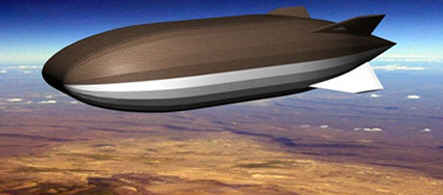
\includegraphics{intro/Stratellite.jpg}
	\captionsource{Airship with non-axisymmetric envelope}{\url{http://www.virtualworldlets.net}}
	\label{Stratellite} %      only if needed 
\end{figure}

Unconventional non-axisymmetric shape provides many advantages over conventional axisymmetric shapes. They can have flatter upper surface and is advantageous for capturing more solar irradiance. Existing literature has good amount of work done on CFD analysis of axisymmetric shapes but not on non-axisymmetric shapes. The reason is obvious, 2D analysis can easily be done for axisymmetric shapes. But to analyse non-axisymmetric shapes, we need to perform 3D CFD analysis. It demands more computational power which might not be available for many researchers. An open source CFD software called OpenFOAM\textsuperscript{\textregistered} (Open source Field Operation And Manipulation) has been used in our present study. OpenFOAM\textsuperscript{\textregistered} comes with an inbuilt meshing (\textit{Block mesh} and \textit{Snappy Hex Mesh}) and post-processing (\textit{Paraview}) utilities, both of which are known for their unique and advanced method of problem solving capabilities. \\

\section{Objective}
The project is divided into two stages namely stage-1 and stage-2. In stage-1, OpenFOAM\textsuperscript{\textregistered} software is validated using existing CFD results available in the literature for four standard shapes. A framework for carrying out multi-disciplinary optimization has been laid out. The framework is then implemented in stage-2 and arrived at an optimal shape with respect to user requirements.
\section{Report layout}
\label{layout}

After providing a brief introduction to shape optimisation outlining the aims and objectives of this study, chapter \ref{literature} gives the detailed literature survey of various fields required for multi-disciplinary shape optimization. Chapter \ref{openfoam} gives a brief introduction about OpenFOAM. Section \ref{Advantages of openfoam} demonstrates the power, advantages and disadvantes of using OpenFOAM\textsuperscript{\textregistered}.
Mesh generation using \textit{SnappyHexMesh} is discussed in section \ref{mesh}. Section \ref{results} validates the OpenFOAM\textsuperscript{\textregistered} software with four axisymmetric standard shapes available in literature. Chapter \ref{geometry}  explains the modified gertler parameter technique used for the parameterization of geometry.

Chapter \ref{optimization} gives a brief overview of need for the surrogate model in the optimisation routine and explains the concept of surrogate model, design of experiments and formulation of different surrogate models. Section \ref{test function} explains the SBDO technique using Himmelblau test function. It also validates the Genetic algorithm code by \cite{Xavier} which is used in subsequent chapters.

Chapter \ref{Surrogate model for CFD} gives the design space and design of experiment study parametres which will be used while building surrogate model in chaper \ref{Training data CFD}. Running the actual CFD simulations for building surrogate model of CFD is done in chapter \ref{Training data CFD}. Chapter \ref{Hoop stress} explains the concept of hoop stress and also gives the methodology to calucate it as given by \cite{alam2017thesis}. The results obtained while performing multi-disciplinary optimisation of aerodynamic drag combined with hoop stress are presented in chapter \ref{Final results}.

\begin{figure}[H]
	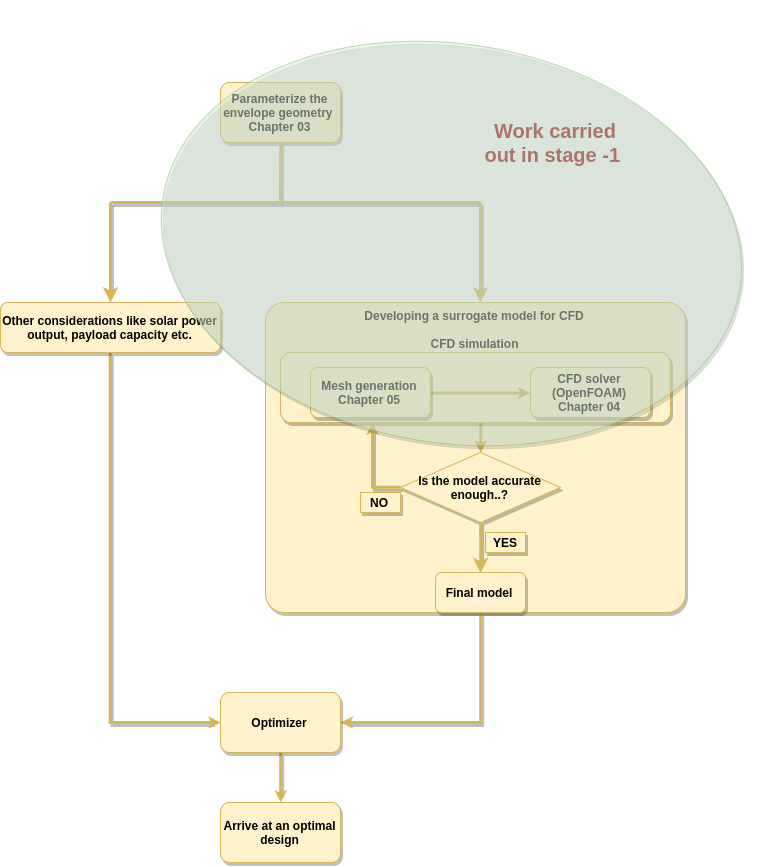
\includegraphics[width=\textwidth]{layout/layout.png} 
	\caption{Framework of multi-disciplinary shape optimization}
	\label{Report layout} %      only if needed 	
\end{figure}
%%
Next Chapter gives brief literature survey that has been carried out to understand the previous research carried out in the field of High Altitude Airships (HAA's) and shape optimisation.


%%% Local Variables: 
%%% mode: latex
%%% TeX-master: "../mainrep"
%%% End: 

%%


%%% Local Variables: 
%%% mode: latex
%%% TeX-master: "../mainrep"
%%% End: 
